\chapter[Experimentos y resultados]{Experimentos y resultados}
\label{ch:exp_result}

\section{Base de datos MMI}
\label{exp:bdd}
Para poder realizar los experimentos con el algoritmo propuesto en el Capítulo~\ref{ch:algoritmo}, se utilizo una base de datos preparada para el reconocimiento facial y de expresiones faciales. Creada por Pantic \etal~\cite{Pantic2005}, MMI es una base de datos multiuso que en esta instancia se utilizo para el reconocimiento de expresiones faciales. Contiene mas de 1000 ejemplos clasificados tanto en imágenes como vídeos; 19 sujetos de prueba; Las edades de los sujetos de prueba varían entre los 19 y los 62 años;  contiene tanto hombres como mujeres, además de tres razas étnicas distintas; Y por ultimo tanto las imágenes como los vídeos están grabados de forma frontal y lateral con respecto al rostro del sujeto. En esta ocasión utilizamos los vídeos grabados de forma frontal, y siendo cada uno de estos etiquetado con una clase distinta para cada expresión facial: Ira(1), Asco(2), Miedo(3), Alegría(4), Tristeza(5) y Sorpresa(6).

\section{Experimentos}
\label{exp:exp}

Para poder probar la efectividad y buen modelado del algoritmo propuesto en el Capítulo~\ref{ch:algoritmo}, se preparo una pila de experimentos, los cuales permitieron realizar una revisión del modelado y precisión de método.
Se prepararon pruebas para cada uno de los pasos del algoritmo, estas pruebas nos permitieron elegir los mejores valores para cada una de las variables a utilizar. Cabe destacar que todos los experimentos realizados sobre el algoritmo, se realizaron en dos instancias de la base de datos MMI, la primera instancia consta de una versión en escala de grises de cada uno de los vídeos, la segunda es una versión a la cual se aplico la técnica LBP descrita en la Sección~\ref{sec:lbp}.

Para la etapa de Extracción de micro-descriptores propuesta en la Sección~\ref{algoritmo:ext_rayos}, se realizaron pruebas que permitieron ver el modelado de los \textit{rayos de flujo} con respecto al movimiento de los pixeles a lo largo de los vídeos, y la elección del tamaño de la Región de soporte $R$ y la Ventana de búsqueda $W$.

En la etapa de Normalización de micro-descriptores, propuesto en la Sección~\ref{algoritmo:normalizacion}, se realizaron pruebas con distintos tamaños de $N$ (Variable utilizada para describir el nuevo tamaño de los \textit{rayos de flujo}) y se realizaron comparaciones con respecto a la Asertividad (Accuracy en ingles) de cada valor.

Para la creación de macro-descriptores, propuesta en la Sección~\ref{sec:macro-descriptores}, se prepararon dos experimentos distintos, primero se realizo un estudio del agrupamiento de los \textit{rayos} en el rostro para cada uno de los vídeos con distintos valores $K$, el cual indica la cantidad de grupos de \textit{rayos de flujo} existen y como se distribuyen en el rostro; el segundo experimento que se realizó fue calcular la Asertividad (Accuracy en ingles) para distintos valores de la variable $K$.

Por ultimo en la etapa de entrenamiento y posterior clasificación, explicada en la Sección~\ref{sec:clasificacion}, se realizaron pruebas con los distintos \textit{Kernel} y sus respectivas variables, los cuales son recibidos por SVM para la generación del modelo.


\definecolor{lightgray}{gray}{0.9}
\newlength{\sz}
\setlength{\sz}{2cm}
\begin{table}[t!]
	\centering
	\begin{tabular}{ >{\centering\arraybackslash}m{.2cm}  >{\centering\arraybackslash}m{1.9cm}  >{\centering\arraybackslash}m{1.3cm}  >{\centering\arraybackslash}m{1.5cm}  >{\centering\arraybackslash}m{1.9cm}  >{\centering\arraybackslash}m{1.3cm}  >{\centering\arraybackslash}m{1.5cm}  }
		\hline\noalign{\smallskip}
		& \multicolumn{3}{ c }{Imágenes sin codificación} & \multicolumn{3}{ c }{Imágenes con LBP}\\
		\hline\noalign{\smallskip}
		\raisebox{.8cm}{\rotatebox{90}{\centering\parbox{2cm}{E1--Ira}}} & 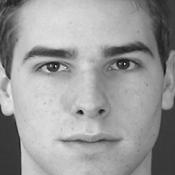
\includegraphics[height=\sz]{Figuras/resultados/E1/E1.png} & 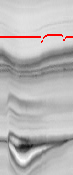
\includegraphics[height=\sz]{Figuras/resultados/E1/E1_YT.png} & 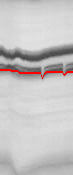
\includegraphics[height=\sz]{Figuras/resultados/E1/E1_XT.png} & 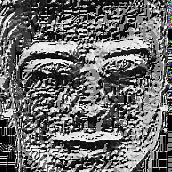
\includegraphics[height=\sz]{Figuras/resultados/E1/E1_LBP.png} & 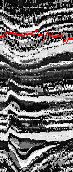
\includegraphics[height=\sz]{Figuras/resultados/E1/E1_LBP_YT.png} & 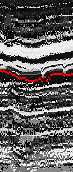
\includegraphics[height=\sz]{Figuras/resultados/E1/E1_LBP_XT.png} \\
		
		\raisebox{.4cm}{\rotatebox{90}{\centering\parbox{2cm}{E2--Asco}}}& 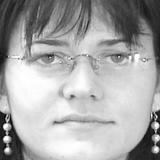
\includegraphics[height=2cm]{Figuras/resultados/E2/E2.png} & 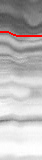
\includegraphics[height=2cm]{Figuras/resultados/E2/E2_YT.png} & 
\includegraphics[height=2cm]{Figuras/resultados/E2/E2_XT.png} & 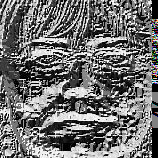
\includegraphics[height=2cm]{Figuras/resultados/E2/E2_LBP.png} & 
\includegraphics[height=2cm]{Figuras/resultados/E2/E2_LBP_YT.png} & 
\includegraphics[height=2cm]{Figuras/resultados/E2/E2_LBP_XT.png} \\
		
		\raisebox{.3cm}{\rotatebox{90}{\centering\parbox{2cm}{E3--Miedo}}}& 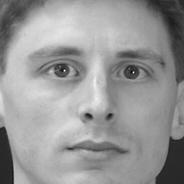
\includegraphics[height=2cm]{Figuras/resultados/E3/E3.png} & 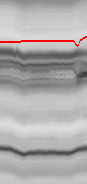
\includegraphics[height=2cm]{Figuras/resultados/E3/E3_YT.png} & 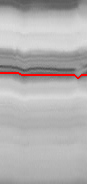
\includegraphics[height=2cm]{Figuras/resultados/E3/E3_XT.png} & 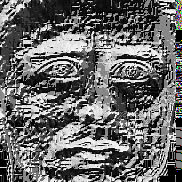
\includegraphics[height=2cm]{Figuras/resultados/E3/E3_LBP.png} & 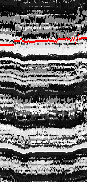
\includegraphics[height=2cm]{Figuras/resultados/E3/E3_LBP_YT.png} & 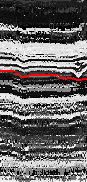
\includegraphics[height=2cm]{Figuras/resultados/E3/E3_LBP_XT.png} \\
		
		\raisebox{.2cm}{\rotatebox{90}{\centering\parbox{2cm}{E4--Alegría}}}& 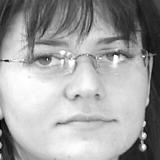
\includegraphics[height=2cm]{Figuras/resultados/E4/E4.png} & 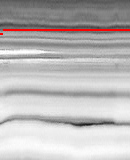
\includegraphics[height=2cm]{Figuras/resultados/E4/E4_YT.png} & 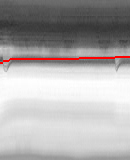
\includegraphics[height=2cm]{Figuras/resultados/E4/E4_XT.png} & 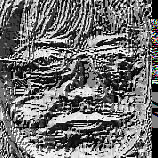
\includegraphics[height=2cm]{Figuras/resultados/E4/E4_LBP.png} & 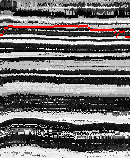
\includegraphics[height=2cm]{Figuras/resultados/E4/E4_LBP_YT.png} & 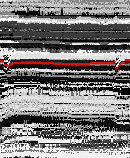
\includegraphics[height=2cm]{Figuras/resultados/E4/E4_LBP_XT.png} \\
		
		\raisebox{0cm}{\rotatebox{90}{\centering\parbox{2cm}{E5--Tristeza}}}& 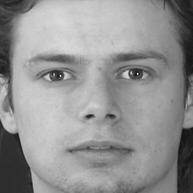
\includegraphics[height=2cm]{Figuras/resultados/E5/E5.png} & 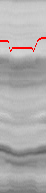
\includegraphics[height=2cm]{Figuras/resultados/E5/E5_YT.png} & 
\includegraphics[height=2cm]{Figuras/resultados/E5/E5_XT.png} & 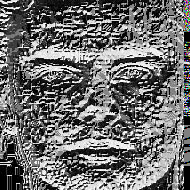
\includegraphics[height=2cm]{Figuras/resultados/E5/E5_LBP.png} & 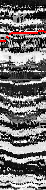
\includegraphics[height=2cm]{Figuras/resultados/E5/E5_LBP_YT.png} & 
\includegraphics[height=2cm]{Figuras/resultados/E5/E5_LBP_XT.png} \\
		
		\raisebox{0cm}{\rotatebox{90}{\centering\parbox{2.1cm}{E6--Sorpresa}}}& 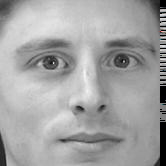
\includegraphics[height=2cm]{Figuras/resultados/E6/E6.png} & 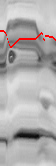
\includegraphics[height=2cm]{Figuras/resultados/E6/E6_YT.png} & 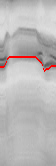
\includegraphics[height=2cm]{Figuras/resultados/E6/E6_XT.png} & 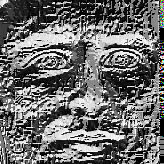
\includegraphics[height=2cm]{Figuras/resultados/E6/E6_LBP.png} & 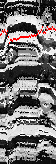
\includegraphics[height=2cm]{Figuras/resultados/E6/E6_LBP_YT.png} & 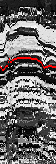
\includegraphics[height=2cm]{Figuras/resultados/E6/E6_LBP_XT.png} \\
		& (a) & (b) & (c) & (d) & (e) & (f) \\

		
	\end{tabular}
	\caption{Tabla comparativa de la extracción de micro-decriptores con vídeos codificados con LBP y sin codificar. Cada fila representa una expresión facial distinta. Las columnas (a) y (d) son el primer cuadro del vídeo, (b) y (e) representan el plano XT, y (c) y (f) representan el plano YT. }
	\label{tabla:comparacion_rayos}
\end{table}


\subsection{Extracción de micro-descriptores}
\label{exp:micro-descriptores}

Etapa propuesta en al Sección~\ref{algoritmo:ext_rayos}, en simples palabras consiste en modelar el movimiento de cada uno de los pixeles a lo largo de todo el vídeo, este modelado es llamado \textit{rayo de flujo}. Para poder extraer un \textit{rayo} se utilizan dos ventanas: la región de soporte y la ventana de búsqueda. Estas regiones permiten calcular a que pixel $(x',y')$ en un tiempo $t+1$ se desplazo pixel $(x,y)$ en un tiempo $t$. Luego de calcular el movimiento de un pixel de $t$ a $t+1$ se crea un \textit{rayo de soporte}, que es la composición mínima para la creación de los \textit{rayos de flujo}. Para ver en detalle este proceso revisar la Sección~\ref{algoritmo:ext_rayos}.

Para poder evaluar el real modelado de los \textit{rayos} sobre el movimiento de los pixeles, se realizo una extracción de los planos $XT$ y $YT$ del vídeo. El plano $XT$ es una imagen extraída del vídeo en un pixel $(x,y)$, donde cada columna representa un cuadro distinto, cada una de estas son extraídas de sus respectivos cuadros $t$, de tal forma que la columna $t$ del plano $XT$ es la fila $y$ del cuadro $t$ del vídeo. Así mismo el plano $YT$ es otra imagen extraída del vídeo en el mismo pixel $(x,y)$, donde cada columna $t$ de este plano representa un cuadro distinto del vídeo, de tal forma que la columna $t$ del plano $YT$ es la columna $x$ del cuadro $t$ del vídeo. Luego de realizar la extracción de los planos y con la posterior obtención del \textit{rayo de flujo} para el pixel $(x,y)$, fue posible realizar un trazado del movimiento del \textit{rayo} en cada una de sus componentes (En el plano $XT$ se trazo el movimiento de la variable $x$ durante los cuadros del vídeo, por el contrario en el plano $YT$ trazo el movimiento de la variable $y$). Ejemplos de estos planos y sus trazos pueden ser vistos en la Tabla~\ref{tabla:comparacion_rayos}, en las columnas (b), (c), (e) y (f).

En general revisando los resultados obtenidos en cada uno de los planos, podemos deducir de forma visual que los \textit{rayos de flujo} modelan de forma aproximada el movimiento de los pixeles. Observando la Tabla~\ref{tabla:comparacion_rayos} y ademas los resultados obtenidos con distintas pruebas, nos dimos cuenta que el modelado de los \textit{rayos} no tiene una mayor variación con respecto a la expresión facial que se esta observando. Al momento de observar las diferencias entre los resultados obtenidos con los videos con codificacion LBP y sin esta, pudimos observar que los \textit{rayos} obtenidos en videos sin LBP obtenian una mejor aproximacion al movimiento real del rayo, este comportamiento puede ser observado al comparar la columna (b) y (e) que represetan la extraccion en el plano $XT$, o comparando (c) y (f) representantes del plano $YT$ en la Tabla~\ref{tabla:comparacion_rayos}. A su vez se puede observar que las componentes de los \textit{rayos} se comportan mejor al modelar los movimientos verticales (Plano $YT$) que los movimientos horizontales (Plano $XT$).

\begin{table}[tb]
	\centering
	\begin{tabular}{ |>{\centering\arraybackslash}m{2.3cm} | >{\centering\arraybackslash}m{1.2cm} | >{\centering\arraybackslash}m{1.2cm} | >{\centering\arraybackslash}m{1.2cm} | >{\centering\arraybackslash}m{1.2cm} | >{\centering\arraybackslash}m{1.2cm} | >{\centering\arraybackslash}m{1.2cm} | }
		\hline
		Codificación & \multicolumn{3}{| c |}{XT} & \multicolumn{3}{| c |}{YT}\\
		\hline
		& & & & & &\\
		Sin codificación & 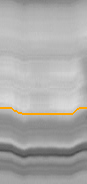
\includegraphics[height=2cm]{Figuras/resultados/comparacion_real/no_lbp/XT/extraido.png} & 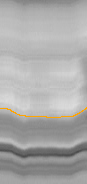
\includegraphics[height=2cm]{Figuras/resultados/comparacion_real/no_lbp/XT/pintado.png} & 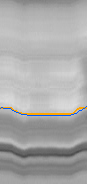
\includegraphics[height=2cm]{Figuras/resultados/comparacion_real/no_lbp/XT/superposicion.png} & 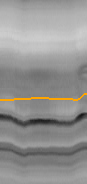
\includegraphics[height=2cm]{Figuras/resultados/comparacion_real/no_lbp/YT/extraido.png} & 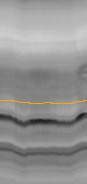
\includegraphics[height=2cm]{Figuras/resultados/comparacion_real/no_lbp/YT/pintado.png} & 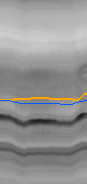
\includegraphics[height=2cm]{Figuras/resultados/comparacion_real/no_lbp/YT/superposicion.png} \\
		
		Codificación LBP & 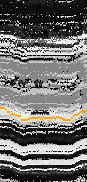
\includegraphics[height=2cm]{Figuras/resultados/comparacion_real/lbp/XT/extraido.png} & 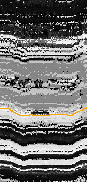
\includegraphics[height=2cm]{Figuras/resultados/comparacion_real/lbp/XT/pintado.png} & 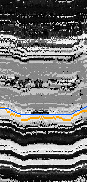
\includegraphics[height=2cm]{Figuras/resultados/comparacion_real/lbp/XT/superposicion.png} & 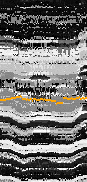
\includegraphics[height=2cm]{Figuras/resultados/comparacion_real/lbp/YT/extraido.png} & 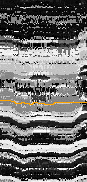
\includegraphics[height=2cm]{Figuras/resultados/comparacion_real/lbp/YT/pintado.png} & 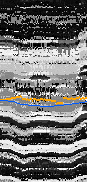
\includegraphics[height=2cm]{Figuras/resultados/comparacion_real/lbp/YT/superposicion.png} \\
		\hline
		& (i) & (ii) & (iii) & (iv) & (v) & (vi)\\
		\hline
	\end{tabular}
	\caption{Tabla comparativa de el calculo del error de cada plano. (i) y (iv) representan el \textit{rayo} extraído por el algoritmo; (ii) y (v) el \textit{rayo} promedio dibujado por las personas; (iii) y (vi) la superposición de ambos (de color amarillo el extraído y color azul el promedio). }
	\label{tabla:comparacion_errores}
\end{table}


Para poder ratificar las observaciones que hemos podido deducir al contemplar el movimiento a través de los planos, se diseño un experimento que nos permitió calcular un error aproximado del modelado de los \textit{rayos de flujo}. Este experimento consistió en pedir a distintas personas que dibujaran el \textit{rayo de flujo} sobre cada plano, para esto utilizaron la herramienta de dibujo paint de Windows. En general se pidió a cada una de las personas que dibujaran como creían ellos que se movía el pixel inicial a lo largo de las texturas representadas en el plano. Luego de esta etapa se procedió a extraer cada una de las componentes de los \textit{rayos} dibujados a mano, con esto se logro calcular un promedio de los trazos de las personas. Este \textit{rayo} promedio es comparado con el extraído por el algoritmo, de tal forma que se puede calcular el error para cada componente y un error general. Este proceso puede ser visualizado en la Tabla~\ref{tabla:comparacion_errores}, donde las columnas (iii) y (iv), representan de forma visual como se superpone un \textit{rayo} sobre otro. El error es obtenido calculando la desviación estándar entre ambas componentes. 

\pgfplotstableset{
  franjas/.style={
    columns/errorG/.style={
      column name=Error,
      precision=1
    },
    every even row/.style={
      before row={\rowcolor{#1}}
    },
    every head row/.style={
      before row=\hline\noalign{\smallskip},after row=\hline
    },
    every last row/.style={
      after row=\hline
    }
  },
  franjas/.default={gray!50},
  tablita/.style={
    columns={rs, ws, errorXT, errorYT, errorG},
    columns/rs/.style={
      column name=$RS$,
    },
    columns/ws/.style={
      column name=$WS$,
    },
    columns/errorXT/.style={
      column name=Error $XT$,
      precision=1
    },
    columns/errorYT/.style={
      column name=Error $YT$,
      precision=1
    },
    franjas,
  }
}

\begin{table}[tb]
	\centering
	\pgfplotstabletypeset[tablita]{Datos/comparacion_NO_LBP.dat}
	\caption{Tabla comparativa de los errores encontrados en los planos $XT$, $YT$ y error general, al calcular los \textit{rayos} con distintos tamaños de ventanas. Sin codificación LBP.}
	\label{tabla:error_no_lbp}
\end{table}

\begin{table}[tb]
	\centering
	\pgfplotstabletypeset[tablita]{Datos/comparacion_LBP.dat}
	\caption{Tabla comparativa de los errores encontrados en los planos $XT$, $YT$ y error general, al calcular los \textit{rayos} con distintos tamaños de ventanas. Con codificación LBP.}
	\label{tabla:error_lbp}
\end{table}

Decidimos utilizar esta métrica de comparación para visualizar como se comportan los \textit{rayos} con respecto al tamaño de las ventanas utilizadas, En las Tablas~\ref{tabla:error_no_lbp}~y~\ref{tabla:error_lbp} se puede ver reflejados los resultados del calculo del error en ambos planos y el error general calculado como el promedio entre ambos errores, utilizando distintos tamaños de ventanas. Con estos resultados logramos darnos cuenta que la idea planteada sobre las diferencias del modelado vertical y horizontal estaba en lo cierto, en ambas tablas podemos ver que el error obtenido en el plano $XT$ es mucho menor al obtenido en $YT$. Ademas en general los errores disminuyen a medida que se aumenta el tamaño de las ventanas $RS$ y $WS$, esto es debido a que mientras mas grande sea la región de soporte, menos probabilidad existe de encontrar otra textura igual en la imagen, por lo cual la probabilidad de encontrar en el siguiente cuadro la textura es mucho mas alta.

\begin{figure}[t]
	\begin{subfigure}{1.0\textwidth}
		\centering
		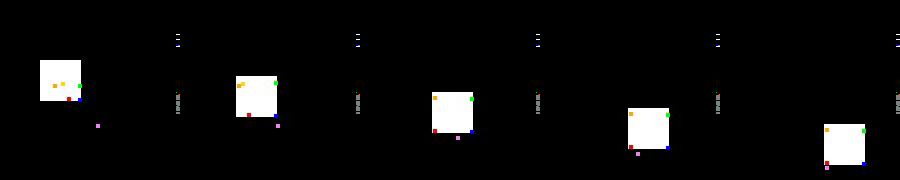
\includegraphics[width=1\textwidth]{Figuras/resultados/videos_sinteticos/v1.png}
		\caption{Vídeo sintético simple sin texturas}
		\label{exp:fig:vs1}
	\end{subfigure}
	
	\begin{subfigure}{1.0\textwidth}
		\centering
		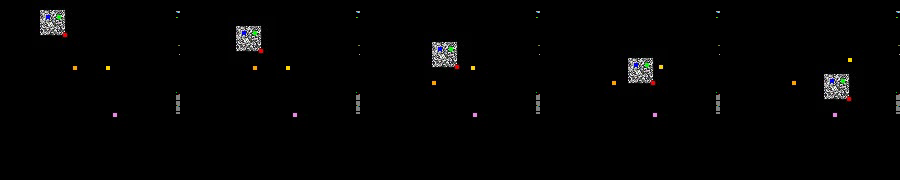
\includegraphics[width=1\textwidth]{Figuras/resultados/videos_sinteticos/v2.png}
		\caption{Vídeo sintético simple con texturas}
		\label{exp:fig:vs2}
	\end{subfigure}
	
	\begin{subfigure}{1.0\textwidth}
		\centering
		\includegraphics[width=1\textwidth]{Figuras/resultados/videos_sinteticos/v3.png}
		\caption{Vídeo sintético con texturas.}
		\label{exp:fig:vs3}
	\end{subfigure}
	\caption{Cortes de vídeos sintéticos, en los cuales se describe el movimiento de ciertos pixeles a los largo del tiempo.} 
	\label{exp:fig:vs}
\end{figure}


Luego de obtener resultados satisfactorios con el modelado de los \textit{rayos de flujo}, decidimos probar si la teoría de extracción de estos podía ser aplicada a otros vídeos y otras texturas, por lo cual preparamos un par de vídeos sintéticos, los cuales describían movimientos predecibles al ojo humano.

Luego de realizar la extracción de \textit{rayos de flujo} a los vídeos generados sistemáticamente, observamos dos fenómenos. Los rayos pueden modelar el movimiento de los pixeles a los largo del tiempo, esto puede ser visto en la Figura~\ref{exp:fig:vs}, en la cual se ven cortes de distintos cuadros de los vídeos y como se mueven sus pixeles. También descubrimos que el modelado de los rayos tiene un comportamiento mas estable cuando existen texturas en las zonas que se están analizando, como se puede ver en las Figuras~\ref{exp:fig:vs2}~y~\ref{exp:fig:vs3}, los pixeles internos del cuadrado siguen durante todo el movimiento en la misma posición del cuadrado, no así en la Figura~\ref{exp:fig:vs1}, en la cual los pixeles que están dentro del cuadrado tienden a juntarse en un punto a medida que el cuadrado se va desplazando.


\subsection{ Normalización de micro-descriptores}


\subsection{ Creación de macro-descriptores}


\subsection{ Entrenamiento y clasificación}


% % % % % % % % % % % % % % % % % % % % % % % % % % % % % % % % % % % % % % % % % % % % % % % % % % % %
% % % % % % % % % % % % % % % % % % % % B O R R A R % % % % % % % % % % % % % % % % % % % % % % % % % %
% % % % % % % % % % % % % % % % % % % % % % % % % % % % % % % % % % % % % % % % % % % % % % % % % % % % 


\subsection{Obtencion del Kernel optimo para SVM}

Hablar sobre lo que se realizo para obtener los mejores valores.

Valores obtenidos para LINEAL y mostrar cuadro y grafico de la variable C v/s Accuracy
Valores obtenidos para RBF y mostrar cuadro y grafico para variable Gamma, C y Accuracy
valores obtenidos para Sigmoid y mostrar cuado de grafico para sus variables
valores obtenidos para Poly y mostrar cuajdro de graficos para sus variables

Hablar de Kernels para Histogramas y hablar de valores obtenidos con el kernel de comparacion de histograma


\subsection{Pruebas sobre variables del algoritmo}
\label{exp:var}
Como se explica en el Capítulo~\ref{ch:algoritmo}, el algoritmo cuenta con tres variables importantes, las cuales son la clave para la eficacia y precisión de este. Estas variables son el tamaño de la \textit{región de soporte} o variable $L$, el valor de la normalización de los \textit{rayos de soporte} o variable $N$ y por ultimo el tamaño del \textit{Bag of Visual Words} o variable $K$.

\subsubsection{Pruebas del tamaño de la región de soporte}
Como se explica en la Sección~\ref{algoritmo:ext_rayos}, la extracción de \textit{rayos}, se utilizan dos estructuras llamadas \textit{región de soporte} y \textit{ventana de búsqueda}, estas son de tamaño $L$x$L$ y $(2L+1)$x$(2L+1)$ respectivamente. El valor de la variable $L$ es muy importante ya que define el tamaño de ambas regiones, y a su vez permite definir el tamaño de la región donde se busca el movimiento de los píxeles, por lo cual un gran tamaño puede indicar mayor precisión y a su vez menor velocidad. La idea de estas pruebas es poder encontrar el valor óptimo de $L$ el cual permita tener una respuesta aceptable por parte del algoritmo. 

\subsubsection{Pruebas de normalización de rayos}	

La normalización de rayos, explicada en la Sección~\ref{algoritmo:normalizacion}, es otro de los procesos a los cuales se debe encontrar un valor óptimo a su variable $N$, esta variable indica cual debe ser el largo de los vectores que representan los \textit{rayos} de los vídeos. El proceso de normalización es un proceso en el cual se requiere llevar todos los vectores al mismo espacio vectorial, para así poder realizar comparaciones entre estos. Este proceso tiene una gran desventaja, esto debido a que al transformar un vector de tamaño mayor a $N$ este tiende a perder información en su compresión, al igual que al agrandar un vector de tamaño menor a $N$ se tiende a agregar información que posiblemente sea falsa o simplemente ruido.

\subsubsection{Pruebas del tamaño del \textit{Bag of Visual Words}}
La técnica de \textit{Bag of Visual Words} utiliza la variable $K$, está representa el numero de \textit{clusters} o grupos que se deben formar en el proceso de creación de la bolsa de palabras, a su vez también indica el tamaño del descriptor final o macro-descriptor que representa a cada vídeo. Esta variable es la  más importante en el algoritmo, esto debido a que una mala elección de la cantidad de \textit{clusters}, puede desencadenar en una mala creación de los macro-descriptores, por lo cual la búsqueda del valor óptimo es muy importante para obtener una buena precisión. La única forma de poder encontrar un valor óptimo o funcional es a través del método de prueba y error, esto debido a que no existe una forma empírica de demostrar cual es el valor óptimo para cada corrida.

